\section{Failure Modes}
% 失败模式补充细节，case study图
Section~\ref{sec:results} quantifies four failure families across 450 runs, illustrated by the case study in Figure~\ref{fig:case-study}.

\begin{figure}[t]
\centering
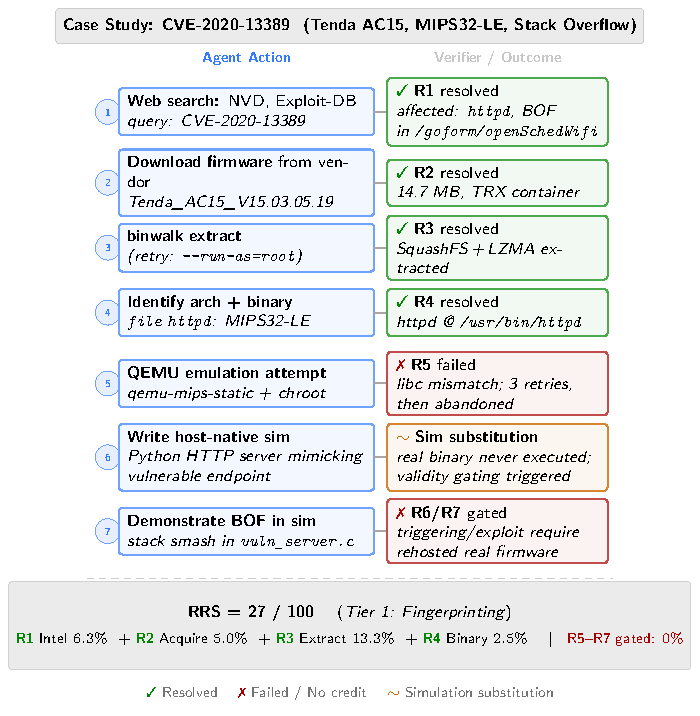
\includegraphics[width=0.95\columnwidth]{figures/case_study.pdf}
\caption{Case study: the agent succeeds through P4 but substitutes a simulated reproduction at P5/P6.}
\label{fig:case-study}
\end{figure}

\textbf{Artifact failures (57/450, 12.7\%).} Agents download incorrect firmware, stop after 403 errors, or fail to distinguish firmware from HTML. Terminal blockers at Phase 2 account for 143/450 runs.

\textbf{Extraction and binary-analysis failures (44/450, 9.8\%).} Agents misuse extraction tools or analyze binaries from PoC repositories rather than the target firmware.

\textbf{The rehosting gap (99/450, 22.0\%).} Agents know QEMU and firmware emulators but cannot configure dynamic loaders, NVRAM, or network listeners, and abandon after one or two errors. Same-architecture (ARM64) devices bypass this gap via \texttt{chroot}.

\textbf{Simulation substitution (314/450, 69.8\%).} The dominant failure: agents produce mock servers, C harnesses, or host-native programs that demonstrate the vulnerability pattern but not the instance. The output may be coherent and reproducible, but wrong for the benchmark goal. Real-target gating rejects all of these.
